\subsubsection{システム構成}
本システムの構成を図\ref{system}に示す.本システムはDjangoで構成されるアプリケーション部(以下,クライアント),およびgolangとdjangorestframeworkで構成されるサーバ部(以下,サーバ)から構築される.
サーバはAPIを用いて統計情報提供機能とコンテナ管理機能を動作させる.コンテンツ提供機能のGUIを図\ref{teikyou}に,統計情報提供機能のGUIを図\ref{toukei}に,コンテナ管理機能のGUIを図\ref{kanri}にそれぞれ示す.

教材提供者は図\ref{teikyou}のコンテンツ提供機能を用いて情報倫理に関するコンテンツを提供する.図\ref{teikyou}の統計情報提供機能では,教材提供者が学習者の回答情報等をグラフとして確認できる.図\ref{kanri}のコンテナ管理機能では教材提供者がDockerを用いて作成した他の教育アプリケーションを本プラットフォームでも利用することが可能となる.

学習者は図\ref{teikyou}のコンテンツ提供機能を用いて作成されたコンテンツを図\ref{naiyou}のようにして閲覧,学習することが可能である.

\begin{figure}[htbp]
    \begin{center}
        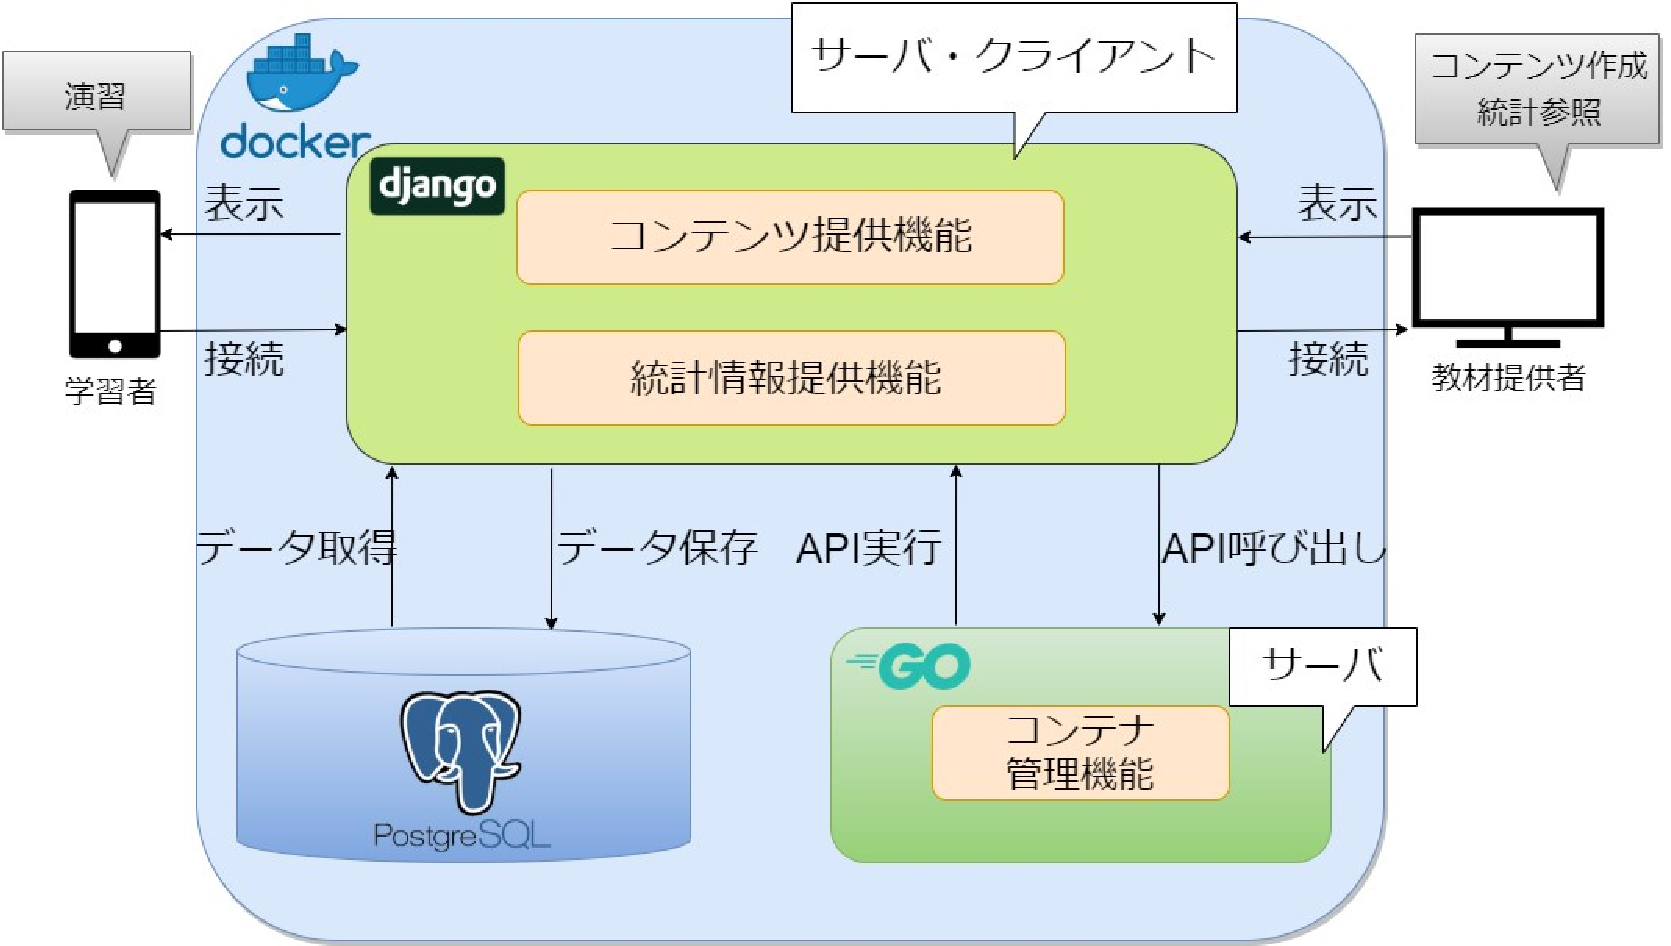
\includegraphics[width=13cm,height=12cm,keepaspectratio]{system-crop.pdf}\\
        %includegraphicsの詳しい使い方ははLaTeXの参考書を参照.
    \end{center}
    \caption{システム構成}
    \label{system}
\end{figure}